\documentclass[ebook,9pt,twoside,final]{memoir}
\usepackage[english]{babel}
\usepackage{amsmath,amssymb,amsfonts,amsthm}
\usepackage{a4wide, graphicx}
\usepackage{listings,endnotes}
\usepackage{hyperref} 
%% to make colored boxes
\usepackage{framed,wrapfig,xcolor}


%% SETUP
\lstset{language=C,basicstyle=\footnotesize\ttfamily} % format verbatime using the c programming syntax
\newcommand{\myindent}{\hspace{0.45cm}}  % home made indent function
\maxtocdepth{section} % only add parts, chapters and sections to toc
\renewcommand{\cftdotsep}{\cftnodots} % remove dots in toc
%\renewcommand{\cftchapterfont}{\mdseries} % toc chapter font 
\chapterstyle{bianchi} % chapter styling
%\addtokomafont{section}{\large} % section font size
%\KOMAoptions{bibliography=totoc,index=totoc} % add bibliography and index to TOC

%% CAPSULE SETUP
\colorlet{shadecolor}{gray!25} 
\renewcommand\FrameCommand{\fboxrule=.4pt,% 
  \fboxsep=2pt\fcolorbox{black}{shadecolor}} 

%% THEOREM SETUP
\swapnumbers % swap theorem numbering
\newtheorem{thm}{Theorem}[section]
\newtheorem{cor}[thm]{Corollary}
\newtheorem{lem}[thm]{Lemma}
\newtheorem{prop}[thm]{Proposition}
\theoremstyle{definition}
\newtheorem{defi}[thm]{Definition}
\newtheorem{exc}{}[chapter]
\newcommand{\ans}[1]{\vspace{0.2cm}\textbf{\ref{#1}}} 


%% BEGIN DOCUMENT
\begin{document}

%% TITLEPAGE
\begin{titlingpage}
\rule[5pt]{155mm}{0.3mm}
\vspace{3cm}
\begin{center}
	\Huge \textsc{Opus Mathematica\\}
	\vspace{2cm}
	\large \textsc{A Complete Guide to the World \\ of Mathematics\\}
	\vspace{10cm}
	\textsc{- Lars Tackmann -\\} \textsc{www.randompage.org}
\end{center}
\end{titlingpage}

%% DEDICATION
\thispagestyle{empty}
\begin{flushright}
This series of books are dedicated to memory of \\ 
Bertrand Russell and Baruch Spinoza whose \\
books taught me the beauty of mathematics \\ 
and made me a lover of philosophy 
\end{flushright}

%% PREFACE
\frontmatter 
\tableofcontents*
\chapter{Preface} 
It has been said that the typical theorem in mathematics states that something you do not understand is equal to something else
you cannot compute. There is a kernel of truth in this joke, since the rigor required when doing mathematical research has found
is way into every nook and corner of every textbook and thereby to a large extend rendered them unreadable to all, except fairly
expert mathematicians; and even these usually disdain from reading such texts cover to cover. The value of mathematical rigor is
not in the question; but such works are condemned to remain works of reference, to be consulted, not read.

This is unfortunate since many people derive great happiness from fiddling with a little mathematics; just consider the many
people who vigorously engages the daily news paper Sudoku puzzel on their way to work. Such spending of time implies that many
people indeed still enjoys the pleasures of the mind. Thus the current crisis in science is to a large extend self inflicted,
modern scientist have done to little to convey what they are doing by hiding behind the often tutted vail of complexity.

However it would be foolish not to acknowledge the complexity of modern mathematical developments, such as Andrew Wiles incredible
proof  of Fermat's Last Theorem or Abel's remarkable proof of the in-solvability of general higher degree equations. Such gems are
usually only available to the person equipped with a sharp mind, a fairly developed bag of mathematical tricks and a certain
intellectual maturity. What I propose here is a book that will build  up enough knowledge as to show the proofs of the greatest
theorems in the history of mathematics;  from Hippocrates Quadrature of the Lune to Lindeman's proof that Pi is Trancendental. I
have sought to make the text completely self contained, so the reader will be taken from the proof that $a^2 + b^2 = c^2$ holds
true for the length of the sides in a right triangle, to the complex proof that if an integer $n$ is greater than 2, then the
equation $x^n + y^n = z^n$ has no solutions for non-zero integers $x$, $y$, and $z$. 

The mathematical mature person is right to ask if such an bold attempt is not futile and that perhaps this author is a bit naive.
Such a question is indeed prudent to ask, but for its answer I need only refer to the massive success of Richard P. Feynman'a
lectures of physics; in which the author successfully conveys such complex matters as Quantum mechanics and General relativity to
people with little other background than a high school education and a lust to learn a little physics. There goes a story that
Feynman was once asked by a Caltech faculty member to explain why spin 1/2 particles obey the Fermi-Dirac statistics. He nodded
and said , "I'll prepare a freshman lecture on it". But a few days later he returned and said. "You know, I couldn't do it, I
couldn't reduce it to freshman level. That means we really don't understand it." 

The text includes a number of exercises along with answers to every one (at least briefly). I am a firm believer in
learning-by-looking, also known as cheating, and thus I encourage the reader to give each problem his best shot, then check the
answer. If correct then move on to a more advanced problem, if not then study the provided solution and try to solve a similar
problem. If you are stuck then don't panic I have included an entire chapter devoted to the fine art of problem solving and
mathematical proof. The exercise are grouped as follows
\begin{itemize}
\item \textbf{Warmups} Problems that everyone should try to solve, even if they appear trivial. As the late great mathematician
George Polya (1887 - 1985) said  "The advanced reader who skips parts that appear too elementary may miss more than the less
advanced reader who skips parts that appear too complex". 
\item \textbf{Study Exercise} Exercises that will develop and widen the ideas from the text, many problems in this section
resembles university exam problems.
\item \textbf{Research Problems} Advanced and interesting problems that may or may not be solvable. These problems provides your
window to mathematical fame, but do not discourage if you fail as at least one person (the author) have failed here before you. 
\end{itemize}
The author will be interested to learn of any solution or headway made into the research problems as well as any simplification or clarification to the non-research ones. The main text will never refer to results developed in the exercises (a very common sin in mathematics), thus every vital result in this book is presented in entirety. This does however not mean that the exercises should be skipped, because in order to understand mathematics you have to do mathematics.

The subject presented here is not laid out in the usual chronological manner, instead I have sought to build up mathematics as a
logical progression of ever more complex ideas. Therefor instead of focusing on historical order I have strived instead to provide
the clearest proofs; so for example, instead of Oresme's original verbal proof of the divergence of the Harmonic Series I have
instead included a never and simpler algebraic proof. At other times the original proof is so beautiful or provide a vital lessons
in mathematical reasoning that I let it's author speak directly (such as Euclid's proof of the Pyteagorian theorem).

The knowledge and proofs contained herein is taken from a multitude of sources, many have been rewritten or reordered so to make
them more accessible, but often one finds mathematics written with such breathtaking clarity as so to render any further attempt
upon simplification impossible. In these cases the information is simply restated and put in context. In the end of each chapter
propper credit is provided as well as suggestions on further reading for the adventures person.\\ 
\\
\indent Mathematics is utility and its usage is spread far and wide; from logical reason about programming languages to the physical sciences. So stories about its usages is included as separate capsules whenever I have found it fitting. At the same time mathematics is also history, from Archimedes war machines used against the intruding romans to everyday stories such as Newton's remark that he "do not like to be teased by foreigners about mathematical things". In the end all that I hope to achieve is to shine a little light on the fascinating field of human creativity known as mathematics, to hopefully illustrate the meaning of the the great philosopher Spinoza's words, when he said that "God is a mathematician". \\
\flushright Lars Tackmann \\ Copenhagen, Denmark\flushleft


%% MAIN BOOK
\mainmatter 
\chapter{Mathematical Foundations}
\section{Elementary Arithmetic and Algebra}
\section{The Art and Craft of Problem Solving}
\subsection{Word Problems}
"A bat and ball, together, cost a total of £1.10 and the bat costs £1 more than the ball. How much is the ball?" The wrong answer
is the one that roughly one in every two people blurts out: 10 pence. The correct answer is 5 pence, since only with a bat worth
£1.05 and a ball worth 5 pence are both conditions satisfied.12

\subsection{Problem Solving Checklist}
\section{Introduction to Mathematical Proofs}
\subsection{Proof by Induction}
\subsection{Proof Checklist}

\chapter{Greek Geometry}
\section{Hippocrates' Quadrature of the Lune}
\section{Euclidian Geometry}
\begin{prop}{\textbf{III.21}}
In a circle, angles in the same segment are equal to one another. 
\end{prop}
\begin{proof} 
Let ABCD be a circle, and let the angles BAD, BED be angles in the same segment BAED; I say that the angles BAD,BED are equal to one another.

For let the center of the circle ABCD be taken, and let it be F; let BF, FD be joined.

Now, since the angle BFD is at the center, and the angle BAD at the circumference, and they have the same circumference BCD as base, therefore the angle BFD is double the the angle BAD. [III. 20] For the same reason the angle BFD is also double the angle BED.

Therefore the angle BAD is equal to the angle BED.

Therefore in a circle the angles in the same segment are equal to one another. $\qedhere$
\end{proof}

\section{Spheres, cylinders and Archimedes}
\section{Euclid in the 21st century}

\chapter{Word Problems (Ramsey Theory)}
- "There are six people in the classroom. Prove that among them  there must be either three people who do not know one another or  three people who all know one another."

- how many people must be invited to a party so that at  least m will know one another or at least n will not know one another.

- How many different   patterns can you create with thread while sewing on a four-hole   button?

\chapter{Topology}
The best example of a manifold is the Earth as portrayed   through a series of maps, each showing only a small part of  its surface. Imagine a map of Manhattan, for example: its Euclidean   nature is obvious. When maps are put together in an atlas,  their parallel lines continue not to cross and their triangles maintain   their 18o-degree nature.

A rubber band can be slipped off any place on a ball, a box, a bun,  or a blob without a hole, which makes them all essentially similar  or, in the language of topology, diffeomorphic to one another. This  means you can reshape any one of them into any other and then  back again.

\chapter{Statistics}
Regression is the main statistical technique used to quantify the relationship between two or more variables. It was invented by
Adrien-Marie Legendre in 1805. A regression analysis would show a positive relationship between height and weight, for example.
If we threw in waistline along with height, we’d get an even better regression to predict weight. The measure of the accuracy of a
regression is called R-squared. A perfect relationship, with no error, would have an R-squared of 1.00 or 100

Strong relationships, like height and weight, would have an R-squared of around 70 percent. A meaningless relationship, like zip
code and weight, would have an R-squared of zero.

The way probability works is that the likelihood of a series of independent events occurring is the multiplication of the
likelihood of each individual event (also known as compound probability). So, if the probability of you finishing this chapter is
9 out of 10 (9/10), and the probability of you finishing the next one is 9/10, the total probability of you finishing both
chapters isn't 9/10: it's 81/100.

%%% EUCLIDIAN GEOMETRY
%%% http://math.furman.edu/~jpoole/euclidselements/eubk3/props.htm

\chapter{Analysis}
\section{Introduction}
Consider in how many ways can we arrange the set $\{1,2,3\}$: 
\[
\{1, 2, 3\}, \{1, 3, 2\}, \{2, 1, 3\}, \{2, 3, 1\}, \{3, 1, 2\}, \{3, 2, 1\}
\]
that is we have $3$ ways of choosing the first element, and $3-1$ options for the second
(as we cannot repeat the first choise) and $3-2$ for the last (as non of the former two choices may be used),
therefor we can arrange them in $3 \cdot 2 \cdot 1 = 6$ ways. In general we define the number of 
permutations of a set with $n$ elements as the faculty function $n!$
\[
n! = n \cdot (n-1) \cdot (n-2) \cdots  (n - (n -1)) = 1 \cdot 2 \cdots n = \prod_{k=1}^{n}k, 
\]

the last notation is new but simply means that we multiply all the values of $k$ from $1$
to $n$. A recursive version (a self-calling function) can be constructed by noting that $n! =
n(n-1)!$. \\

\myindent Now consider a slightly more complex question: in how many ways can we pick two 
elements from the set $\{1,2,3\}$, the answer turns out to be three ways: 
\[
\{1, 2\}, \{1, 3\}, \{2, 3\}
\]
To generalize this we can ask in how many ways can we pick a unordered subset with $k$ elements from a set with $n$
elements ?. To answer this, observe there are $n$ choices for the first element and for each of these there are 
$n - 1$ choices for the second; and so on until there are $n - k + 1$ for the k'th and thus $n(n-1) \cdots (n - k + 1)$ 
choices for picking a $k$-element sequence from $n$. Now since each $k$-element subset has exactly $k!$ different 
orderings, we get our answer by dividing with $k!$:
\begin{equation}\label{binom}
\binom{n}{k} = \frac{n(n-1) \cdots (n - k + 1)}{k!},  \qquad \text{integer } n \geq k \geq 0
\end{equation}
and if we multiply the numerator and denominator of \ref{binom} by $(n - k)!$ we get:
\[
\frac{n(n-1) \cdots (n - k + 1)}{k!} \cdot \frac{(n - k)!}{(n - k)!} =  \frac{n!}{k!(n-k)!}
\]
The symbol $\binom{n}{k}$ is known as a binomial coefficient and we read it "$n$ choose $k$". Using this result we can
calculating the above question about choosing two elements from a three element set as:
\[
\binom{3}{2}  = \frac{3!}{2! (3-2)!} = \frac{3 \cdot 2 \cdot 1}{2 \cdot 1 \cdot 1} = 3
\]
Interestingly when determining the number of ways to pick $k$ elements we have in effect also specified the $n-k$
unchosen things, therefore 
\begin{equation}\label{binom_symmetry}
\binom{n}{k} = \binom{n}{n-k} 
\end{equation}
this symmetry can be observed in the above example where we have $3$ ways of picking $2$ elements from a $3$-element set
but then also $3$ ways of picking the remaining element. It also follows directly from the definition of the binomial
coefficient 
\[
\binom{n}{k} =  \frac{n!}{k!(n-k)!} =  \frac{n!}{(n-(n-k))!(n-k)!} = \binom{n}{n-k}
\]

\myindent Another rather remarkable result, known as Pascal's rule, can be derived by marking a particular object
$\epsilon$ in an $n$-element set. Now if we pick $k$ objects from $n$, then either $\epsilon$ is picked or it is not. If
$\epsilon$ is in the subset then there is $k-1$ objects left to choose among the $n-1$ elements, or more formally
$\binom{n-1}{k-1}$. If $\epsilon$ is not in the subset, we need to choose all the $k$ elements in the subset from the
$n-1$ objects that are not $\epsilon$; formally that is $\binom{n-1}{k}$. Thus there are 
\[
\binom{n-1}{k-1} + \binom{n-1}{k}
\]
ways to choose $k$ elements from $n$ depending on whether $\epsilon$ is included in each selection or not. But this
number must be the same as the binomial coefficient and thus we get: 
\begin{equation}\label{pascal_rule}
\binom{n}{k}  = \binom{n-1}{k-1} + \binom{n-1}{k}
\end{equation}
Those who consider the above reasoning a bit vague may rejoice from the following straightforward algebraic manipulation
\begin{align*}
 \binom{n-1}{k-1} + \binom{n-1}{k} 
& =  \frac{(n-1)!}{(k-1)!((n-1)-(k-1))!} + \frac{(n-1)!}{k!((n - 1) - k)!} \\
& =  \frac{(n-1)!}{(k-1)!(n-k)!} + \frac{(n-1)!}{k!(n - (k + 1))!} \\
& =  \frac{k(n-1)!}{k!(n-k)!} + \frac{(n-1)!(n-k)}{k!(n - k)!} \\
& =  \frac{(n-1)!(k + n - k)}{k!(n-k)!} \\
& =  \frac{n!}{k!(n-k)!} 
\end{align*}
It is interesting to notice that in the field of combinatorics we can arrive at the same result in different ways.
Indeed the smart mathematician should always seek alternate routes whenever a result causes the least headache.

%% CAPSULE
\begin{framed}
\begin{wrapfigure}{r}{0pt}
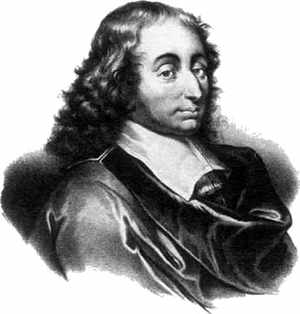
\includegraphics[width=4cm]{images/blaise_pascal.jpg}
\end{wrapfigure} 
\textbf{Blaise Pascal} ($1623-1662$)\\ French mathematician, physicist, and religious philosopher. He
was a child prodigy who already at the age of sixteen was corresponding, by letter, with the mighty Rene Descartes
($1596-1650$). When Descartes later leaned the age of Pascal he refused to believe that so young a boy was the author of
such brilliant mathematics. 

\myindent Pascal, like Newton, was a devoted theologist who spend most of his life pondering religious questions instead
of mathematical ones. By studying omens in the events around him he in fact ended up dropping mathematics completely,
since he found it apparent that God's plan for him did not include mathematics. But at the age of $35$ Pascal observed
that a particular nagging toothache seamed to go away when he pondered about mathematical things.  He concluded that
this was a good omen and thus spend one week in hectic mathematical activity. He never returned to mathematics after
this and died at the age of 39. 

\myindent Even with such a short and unfocused scientific career, Pascal managed to do become a first rate scientist. He
made important contributions to the construction of mechanical calculators, the study of fluids, and clarified the
concepts of pressure and vacuum. Pascal also helped create two major new areas of research. He wrote a significant
treatise on the subject of projective geometry and later corresponded with Pierre de Fermat on probability theory.
\end{framed}


%% PASCALs TRIANGLE
\myindent From Pascal's rule we can construct his famous triangle. Observe that according to this rule (see \ref{pascal_rule}) you can calculate $\binom{5}{3}$ as:
\begin{align*}
 \binom{5}{3}
& =  \binom{4}{3} + \binom{4}{2}  \\
& =  \binom{4}{3} + \binom{3}{2} +  \binom{3}{1} \\
& =  \binom{4}{3} + \binom{3}{2} +  \binom{2}{1} + \binom{2}{0} \\
\end{align*}
as $\binom{2}{0} = 1$, we can stop the expansion. In general as $\binom{n}{n}$ and $\binom{n}{0}$ are always
$1$ (when $n \geq 0$) we are guarantied that the expansion always terminates. Thus we have found a convenient way of
expressing higher binomial coefficients as sums of consecutive smaller ones:\\ 
\begin{center}
\begin{tabular}{l|*{5}{c}r}
\toprule
$n$ & $\binom{n}{0}$        & $\binom{n}{1}$ & $\binom{n}{2}$ & $\binom{n}{3}$ & $\binom{n}{4}$  & $\binom{n}{5}$ \\
\hline
0		& 1                     & 0 			       & 0 			        & 0 			       & 0 			         & 0   \\
1   & 1                     & 1 			       & 0 			        & 0 			       & 0  			       & 0   \\
2   & 1                     & 2 			       & 1 			        & 0 			       & 0  			       & 0   \\
3		& 1                     & 3 			       & 3 			        & 1			         & 0  			       & 0   \\
4		& 1                     & 4 			       & 6 			        & 4			         & 1  			       & 0   \\
5		& 1                     & 5 			       & 10 			      & 10			       & 5  			       & 1   \\
\bottomrule
\end{tabular}
\end{center}
discarding the zero's we can arrange these numbers into a triangle: 
\[
\begin{array}{c} 
1 \\ 
1\ \myindent 1\\ 
1\ \myindent 2\ \myindent 1   \\ 
1\ \myindent 3\ \myindent 3\   \myindent 1   \\ 
1\ \myindent 4\ \myindent 6\   \myindent 4\   \myindent 1\\ 
1\ \myindent 5\ \myindent 10\ \myindent 10\ \myindent 5\ \myindent1\\
\ \textnormal{and so on} \ \\
\end{array} 
\] 
where the next row must contain:
\[
\binom{6}{0} \myindent \binom{6}{1} \myindent \binom{6}{2} \myindent \binom{6}{3} \myindent \binom{6}{4} \myindent \binom{6}{5} \myindent \binom{6}{6} 
\]
but we already know that expressions like $\binom{6}{1}$ can be rewritten to $\binom{5}{1} + \binom{5}{0} = 5 + 1$. So we see that each entry in the new 
row is obtained simply by adding the numbers in the row above to the left and right.
\[
1\ \myindent 6\ \myindent 15\ \myindent 20\ \myindent 15\ \myindent 6\ \myindent 1
\]

\newpage
%%
\section{Newton's Binomial Theorem}
In mathematics a binomial is a polynomial with two terms, i.e such as these
\[\begin{array}{lcl} 
(a + b)^0 &=& 1\\
(a + b)^1 &=& a + b \\
(a + b)^2 &=& a^2 + 2ab + b^2 \\
(a + b)^3 &=& a^3 + 3a^2b + 3ab^2 + b^3 \\
(a + b)^4 &=& a^4 + 4a^3b + 6a^2b^2 + 4ab^3 + b^4 \\
:                &   & :
\end{array}\]
or in general 
\[
(a+b)^n = \overbrace{(a+b)(a+b)\cdots(a+b)}^{n\textnormal{ factors}}
\]
the relationship between such polynomials and combinatorics stems from the so called binomial theorem.  


%% EXERCISES
\newpage
\section*{Exercises}
\addcontentsline{toc}{section}{Exercises} 
\subsection*{Warmups}
% 1
\begin{exc}\label{ex:analysis:1}
Show that 
\[
\binom{n}{0} + \binom{n}{1} + \cdots + \binom{n}{n - 1} + \binom{n}{n} = 2^n
\]
\end{exc}
% 2
\begin{exc}\label{ex:analysis:2}
Find a simple sum expressing the difference between the sum of the squares and the square of the sums. i.e.:
\[
(a + b + \cdots)^2 - (a^2 + b^2 + \cdots) = ?
\]
Then use it to find the difference between the sum of the squares of the first one hundred natural numbers and the
square of the sum (\textbf{note} you should be able to do this without a calculator). 
\end{exc}

%% TODO books used
%% - Concrete mathematics (chapter on binomials)
%% - iJourney Through Geneious (chapter on Newton)

\chapter{Elementary Number Theory}

%% BASICS
\section{Basic Properties}
In number theory we deal with the properties of various classes of numbers such as the integers, which is any number that can be written without a fractional or decimal component and is denoted with the the symbol $\mathbb{Z}$. Thus, $-7$, $0$, and $2$ are integers; $1.7$ and $\frac{1}{7}$ are not. Incidentally the Latin word "integer" literally means "untouched", hence "whole". Of particular interests is the set of all positive integers, also known as the natural numbers and symbolized by $\mathbb{N}$. However before we immerse ourself in the exciting properties of natural numbers let us first consider that integers are either $even$ or $odd$, more formally we write: 
\begin{defi}\label{num_def}
The $even$ numbers are the numbers written on the form $2k$ and the $odd$ numbers are the numbers written on the form $2k+1$ where $k$ is any integer.
\end{defi}
some arithmetic can be used to check that this indeed yields the desired numbers:
\[\begin{array}{lcl} 
2 \cdot 0     & = & 0 \\
2 \cdot 0 + 1 & = & 1 \\
2 \cdot 1     & = & 2 \\
2 \cdot 1 + 1 & = & 3 \\
:             &   & :
\end{array}\]

The $odd$ numbers may also be expressed as being either one more than a multiple of $4$ or three more than a multiple of $4$. Symbolically, we can say that they are either of the form $4k + 1$ or of the form $4k  + 3$. Again some examples clarifies the smoke
\[\begin{array}{lcl} 
4 \cdot 0 + 1 & = & 1 \\
4 \cdot 0 + 3 & = & 3 \\
4 \cdot 1 + 1 & = & 5 \\
4 \cdot 1 + 3 & = & 7 \\
:             &   & :
\end{array}\]

incidentally this shows that when we divide a $odd$ number by $4$, we must get a remainder of either $1$ or
$3$ \label{remainder}. Armed with this knowledge we can shine some light on the properties of $odd$ numbers:
\begin{cor}
The square of an $odd$ number is $odd$
\end{cor}
\begin{proof}
Consider, by \ref{num_def}, the algebraic form of the square of an odd number
\[\begin{array} {lcl} 
(2k+1)^2 & = & (2k)^2 + 2(2k) + 1 \\ 
                 & = & 4(k^2 + k) + 1 
\end{array}\]
The last expression being on the form $4k + 1$ yields the desired result. 
\end{proof}

Integers can be used to construct another class of numbers, known as the rational numbers. Here we say a 'rational
number' is a fraction $\frac{a}{b}$, where $a$ and $b$ are integers; we may suppose that $a$ and $b$ have no common
factor (since if the had we could remove it) and that $b$ does not equal zero. We denote these numbers by $\mathbb{Q}$
for quotient

\myindent With only these properties at hand we can move on to prove one of mathematics first great results; that
$\sqrt{2}$ is irrational. To say that something is irrational is merely they same as saying that it cannot be written on
the form $\frac{a}{b}$. This may sound simple, yet it is not immediately clear that such numbers should even exists. The
ancient greek mathematician Pythagoras believed that all numbers were rational, so it was an unwelcome fact when one of
his students Hippasus proved the existence of irrational numbers. As the story goes, Pythagoras took Hippasus far out to
sea and threw him in the ocean, left to die for his discovery of these ungodly numbers.  
\begin{prop}
$\sqrt{2}$ is irrational.
\end{prop}
\begin{proof}
To say that $\sqrt{2}$ is irrational is then the same as saying that $2$ cannot be expressed in the form
$\left(\frac{a}{b}\right)^2$ or that the equation 
\begin{equation}\label{2_irrational}
a^2 = 2b^2
\end{equation}
cannot be satisfied by integral values of $a$ and $b$ without any common factor. Let us for sake of eventual
contradiction suppose that \ref{2_irrational} is true for some $a$ and $b$, then it follows that $a^2$ is even (since
$2b^2$ is divisible by $2$) and thus that $a$ is even (since the square of an odd number is odd). If $a$ is even then
\[
a = 2c
\]
for some integral value of $c$; and therefore
\[
 a^2 = 2b^2 = (2c)^2 = 4c^2
\]
or
\[
b^2 = 2c^2
\]
Hence $b^2$ is even and therefor $b$ is even. Now since both $a$ and $b$ are even they must have the common factor $2$.
This contradicts our hypothesis, and therefore the hypothesis is false 
\end{proof}
Notice how this proof is by  \emph{reductio ad absurdum}, a proof style much beloved by the greeks and one of
mathematics finest weapons. In these types of proofs we attack our theorem by taking an assumption and then show that it
leads to a contradiction and hence is false. 

\myindent Now since we have proved that $\sqrt{2}$ cannot be written as a fraction can we then find another way to express it ?. By definition, a number is $algebraic$ (denoted by $\mathbb{A}$) if it is the solution to some polynomial equation
\[
a_{n}x^{n} + a_{n-1}x^{n-1} + \cdots + a_{2}x^{2} + a_{1}x + a_0 = 0 
\]
where all the coefficients $a_n, a_{n-1}, \cdots, a_2, a_1$ and $a_0$ are integers. Now as $\sqrt{2}$ is the solution to the polynomial $x^2 - 2 = 0$ it follows that it is a irrational algebraic number. Also as any integer $k$ is a solution to $x-k=0$ we see that all integers are algebraic and hence $\mathbb{Z} \in \mathbb{A}$. Later we shall meet another class of numbers known as transcendental numbers  $\mathbb{T}$ which is simply the set of all non-algebraic numbers. As it turns out almost all irrational numbers are transcendental and all transcendental numbers are irrational. The box below should hopefully clarify the relationships between these various sets of numbers
\begin{figure}[htb!]
\begin{center} 
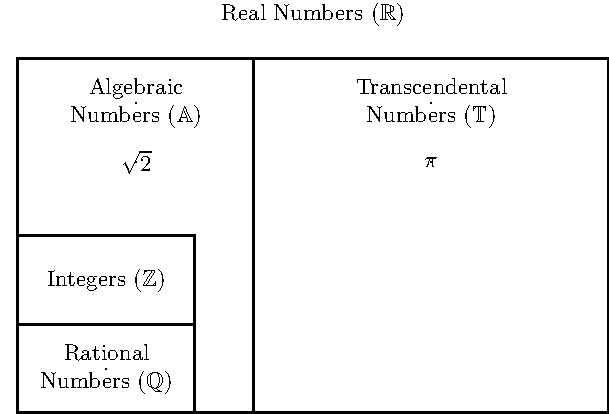
\includegraphics[width=10cm]{images/number_types.pdf}
\end{center}
\end{figure}

Note how all of these numbers are contained in the set of real numbers $\mathbb{R}$.  The real numbers thus includes both integers and rational numbers, such as $42$ and $\frac{1}{3}$, and transcendental numbers, such as $\pi$ and irrational algebraic numbers such as $\sqrt{2}$. Informally we may think of real numbers as any number with or without a decimal point that may contain an infinite decimal tail that continue in some way.
%%  CAPSULE
\begin{framed}
\textbf{Constructible Numbers}\\ A number is said to be constructible if it can be represented by a finite number of additions, subtractions, multiplications, divisions, and square root extractions of integers. Such numbers correspond to line segments which can be constructed by beginning with a unit length (that is, a length to represent the number "$1$") and keep track of what  other lengths we can produce by straightedge and compass construction.

\myindent It turns out that the totality of all possible constructible lengths, while vast, does not include every real number; as it can be shown that all constructible numbers are algebraic it follows that no transcendental numbers can be constructed. However integers such as $1,2,3$ and rationales such as $1/2, 1/3, 1/4$ and square roots, like $\sqrt{2}$ and $\sqrt{5}$ can all be constructed. Further, if we can construct two  magnitudes, we can construct their sums, difference, product and quotient and thus even complex expressions such as
\[
\sqrt{\frac{2+\frac{1}{13}\sqrt{3}}{1 + \sqrt{4 + \sqrt{3}}}}
\]
are actually constructible.
\end{framed}

Now that we have tasted the various flavors of numbers, let us return to theory of numbers and the exciting concept of divisibility.



%% DIVISIBILITY 
\section{Divisibility}
The integer $n$ is divisible by $m$ if the ratio $n/m$ is an integer. Hence we write $m|n$ when $m$ divides $n$ evenly and define
\begin{equation}\label{divisibility}
m|n \Longleftrightarrow m > 0 \textnormal{ and } n = mk \textnormal{ for some integer } k
\end{equation}

How do we know if a number is divisible by some other number ?. Here we are out of luck, in general we can only answer
this by doing full division and checking if the remainder is zero. Mathematics contains many functions that are easy to
do (such as multiplication and differentiation) but hard to undo (such as division and integration). Later on we will
see that exactly this property of division can be used to craft a simple scheme for secure communication. For now
let us consider what properties we can extract from the above definition of divisibility.
\begin{prop}
If $a > b$ and $n$ divides $a$ and $b$ evenly then it also divide their difference.
\end{prop}
\begin{proof} 
By \ref{divisibility} we have $a = nx$ and  $b = ny$ for some integral value of $x$ and $y$. Thus $a-b = nx - ny =
n(x-y)$ as desired.\qed
\end{proof}

As remarked on page \pageref{remainder} not all numbers divides evenly: 
\begin{prop}\label{division_algorithm}
If $a$ and $b$ are integers with $b\neq0$, then there is a unique pair of integers $q$ and $r$ such that
\[
a = qb+r \textnormal{ and } 0 \leq r \leq |b| 
\]
\end{prop}
Note that 
\[
\frac{a}{b} = q + \frac{r}{b}  
\] 
where for $b>0$ we have $0 \leq \frac{r}{b} < 1$ and for $b<0$ we have $0 \geq \frac{r}{b} > -1$. As example the
division $9/4$ with $a=9$ and $b=4$ becomes $9=2\cdot4 + 1$ giving us the quotient $q=2$ and remainder $r=1$
\begin{proof}
Our job is to prove that the numbers $q$ and $r$ exists, known as existence and that they are unique, also known
as uniqueness. First we prove existence. Let
\[
S = \{a-nb|n \in \mathbb{Z}\} = {a,a \pm b,a \pm 2b,...}
\]
\qed
\end{proof}

\subsection{Euclid's Algorithm}
Euclid devised a cleaver algorithm for locating the greatest common divisor. 



%% PRIMES
\section{Primes}
The \textit{prime numbers} or \textit{primes} are the numbers
\[2,3 , 5, 7, 11, 13, 17, 19, 23, 29, 31, 37 ...\]
which cannot be resolved into smaller factors\endnote{There are technical reasons for not counting 1 as a prime}. The primes are the material out of which
all numbers are build up by multiplication: thus $666 = 2 \cdot 3 \cdot 3 \cdot 37$, indeed the following holds true:

\begin{prop}\label{prim_div}
Every integer n $>$ 1 is divisible by atleast one prime
\end{prop}
\begin{proof} 
Let $A$ be a composite number (i.e. non prime). By defenition there must be some smaller number $B$ dividing evenly into $A$, where 1 $<$
$B < A$. Now either $B$ is prime or it is not. If $B$ is prime, then the original number $A$ indeed has a prime divisor, as claimed. Otherwise, $B$ is not
prime and so has a divisor, say $C$, with $1 < C < B <$ A. If $C$ is prime, we are done, for $C$ divides evenly into $B$, and $B$ divides evenly into $A$.
If $C$ is composite then it must have a propper divisor, $D$, and thus we continusly arrive at:
\[
A > B > C > D > ... > 1
\]
But all of these are positive integers, so we must reach a point in which we find a prime. Therefor any number, which is not prime itself, is divisible
by at least one prime (usually, of cause, by several).
\end{proof}

If one surveys the list of the first 50 primes
\begin{lstlisting}
2, 3, 5, 7, 11, 13, 17, 19, 23, 29, 31, 37, 41, 43, 47, 53, 59, 61, 
67, 71, 73, 79, 83, 89, 97, 101, 103, 107, 109, 113, 127, 131, 137, 
139, 149, 151, 157, 163, 167, 173, 179, 181, 191, 193, 197, 199, 
211, 223, 227, 229
\end{lstlisting}

then apparently the primes seams to be getting scarcer as the numbers go larger. Indeed between the numbers $1$ and $1000$ there are $168$ primes, whereas between $9000$ and $10.000$ there is but $112$. At first this seams logical enough since small numbers only have few possible factors and thus higher likelihood of being primes, yet one cannot help ask if we will ever reach such large numbers that the primes may eventually run out completely, rendering all subsequent numbers composite. Luckily this question had already been answered by the great greek mathematician Euclid who 300 B.C. in his IX book as proposition 20 (IX.20) indeed claimed:

\begin{prop}
Prime numbers are more than any assigned multitude of prime numbers.
\end{prop}
Euclid's terminology seams somewhat strange, what he is really proposing is that the sequence of primes does not end.
\begin{proof}
Let us for sake of eventual contradiction suppose that there is only a finite number of primes and that
\[
2, 3, 5, ..., P
\]
is the complete series (so that $P$ is the largest prime); and let us, on this hypothesis, consider the number $Q$ defined by the formula
\[
Q = (2 \cdot 3 \cdot 5 \cdots P) + 1
\]
It is plain that $Q$ is not divisible by any of $2, 3, 5, ..., P$; for it leaves the remainder $1$ when divided by any one of these numbers. But, if $Q$ is not  prime, then by \ref{prim_div} it is divisible by some prime, and therefore there is a prime (which may be $Q$ itself) greater than any of them. This contradicts our hypothesis, that there is no prime greater than $P$; and therefore this hypothesis is false.
\end{proof}

Finding and counting the primes is a long standing hobby for mathematicians, and one might ask if it can be automated. One such method was discovered by the greek mathematician Eratosthenes (ca. 284-192 B.C.) who as the chief librarian at the great Library at Alexandria spend much of  his time studying mathematics, astronomy and philosophy. His method (known as Eratosthenes sieve) is as follows; write a list of all the consecutive integers, starting with $2$, among which you want to find the primes. As $2$ is prime, cross all subsequent multiples off. The next integer that has not yet been crossed of (3) must then also be prime and so we can eliminate all of its multiples. As we continue in this manner we will clearly sieve out all composite numbers and be left with the primes.
\begin{verse}\emph{
Sift the Twos and sift the Threes,\\
The Sieve of Eratosthenes.\\
When the multiples sublime,\\
The numbers that remain are Prime.}
\end{verse}
although this method will indeed generate the primes, it is not as efficient as one might have liked (although optimized and more complex methods exists). Later we shall encounter the prime counting function $\pi(n)$,  which outputs the number of primes less than or equal to a given number $n$ (the use of $\pi$ in this function is an unfortunate standard as it has nothing to do with the constant $3.1415...$).


\section{Fermat's Little Theorem}


%% EXERCISES
\newpage
\section*{Exercises}
\addcontentsline{toc}{section}{Exercises} 
\subsection*{Warmups}
% 1
\begin{exc}\label{ex:elem-num:1}
In 2000 the Jordanian mathematician, Murad A. AlDamen\endnote{Found on the prime puzzlers project, at: \emph{http://www.primepuzzles.net/puzzles/puzz\_101.htm}} devised the following method for testing divisibility
\begin{enumerate}
\item Use Murad's method to answer the following: does $61$ divides $3598207$ ?
\item Prove Murad's method.
\end{enumerate}
\end{exc}

%% ENDNOTES
\theendnotes

%% FROM Mathematics
Numbers that can be obtained by raising 2 to a power and then subtracting 1 are called Mersenne numbers, for reasons I’ll give later in the chapter. Prime numbers of this particular form are called Mersenne primes 

fundamental theorem of arithmetic: that every natural number greater than 1 is either prime, or else can be expressed as a product of primes in a way which is unique except for the order in which the primes are arranged.

the prime numbers are the basic building blocks from which all the natural numbers are constructed.

%% TODO
%% Of particular interest in the non-negative integers i.e. elements of the set $\{0,1,2,3...\}}$, also known as the natural numbers and usually abbreviate as $\N$.
%% - Fermat capsule (and his claims)
%% - Euler capsule (and his teachers)
%% - phi and e are irrational
%% - prime counting function
%% - eliptic curves
%% - enhanced prime finding and locating algorihms (sqare root of n}
%% - one way functions and cryptography (RSA - the code book)

\chapter{Curious and Interesting Numbers}
\section{Numerous Curiosities}
\subsection{Perfect Numbers} 
A number which is the sum of all its digits is said to be perfect, (Euclid IX.36)

\section{Fibonacci Numbers}
The Fibonacci sequence of numbers is a pleasantly simple class of numbers and perhaps the mathematical device most 
frequently used in nature. The first few numbers are
\begin{center}
\begin{tabular}{c|*{11}c}
$n$      & $0$ &  $1$   & $2$ &  $3$ & $4$ & $5$ & $6$ & $7$  & $8$    & $9$   & $10$ \\
\hline
$F_n$ & $0$ &  $1$   & $1$ &  $2$ & $3$ & $5$ & $8$ & $13$ & $21$ & $34$ & $55$ 
\end{tabular}
\end{center}

They are defined by the requrence:
\[\begin{array}{lcl} 
F_0 & = & 0 \\
F_1 & = & 1 \\
F_n & = & F_{n-1} + F_{n-2}
\end{array}\]
a simple recurence which simply ensures that every Fibonacci number is the sum of the two previous ones.

Fibonacci numbers have some intersting propertie, observing the list above one is tempted to conclude that every 3rd
number is even:
\begin{proof}

\end{proof}

inspecting the sum of the first $n$ Fibonacci numbers suggests TODO
\begin{proof}
We will attempt a proof of $\sum_{k=1}^{n} = F_{n+2} - 1$ by induction
\end{proof}

\myindent One thing you quickly release when computing Fibonacci numbers is that there is a whole lot of computation going on, due
to the repeatet double recursive calls. A tail-recursive function is a function which only have one recursive call, this
property makes them easier to handle and often faster to compute so lets attempt to remove one of the recursive calls


\subsection{Generating Functions}
One might ask if we can perhaps remove these calls and compute the numbers directly. 

\chapter{Geometry}
\section{Analytical geometry}
\section{Elliptic geometry}
\section{Hyperbolic geometry}

\chapter{Set theory}

\section{Naive set theory}
\section{Counting the Infinite}
\subsection{Problems with naive set theory}
\section{Axiomatic set theory}
\section{Cantor and the Transfinite Realm}

\chapter{Logic}

\section{Incompleteness}

%% APPENDIX
\appendix
\chapter{Answers to Exercises}
Each exercise is numbered in accordance with the chapter where it is to be found and thus exercise $2$ in chapter $1$ is referenced as $1.2$.\\ 

%% BASIC CHAPTER
\ans{ex:analysis:1} Realizing that $2^n = (1 + 1)^n$ gives 
\[
(1 + 1)^n = \binom{n}{0}1^n + \binom{n}{1}1^{n - 1}1 + \cdots + \binom{n}{n - 1}1*1^{n - 1} + \binom{n}{n}1^n
\]
and since 1 to any power is 1, we get the desired result.

\ans{ex:analysis:2} TODO

\ans{ex:elem-num:1}  TODO


Let L*M=N =n1+10n2, L(k1+10k2)=n1+10n2

L*k1-n1=10a �.(1)

-10Lk2=10a-10n2, Lk2=a-n2

n2 �Lk2=a � (2)

add one to two and by N=M*L

we find ((n1+10n2)(k1-k2)+ (k1+10k2)(nn-n1))/(k1+10k2)=11a, then (n2k1-k2n1)=0 (mod M)
 
%% use \gls{} or \Gls to reference singular names
% use \glspl or \Glspl to reference plural names

% TODO missing from glossary
% Domain and CoDomain
% Sujective, Bijective and injective
% Monomial, binomial, polynomial
% Quadratic equations
% Product, Factors
% DC
% DB
%* Cashflow
%* PV
%* PMT
%* FV
%* Principle (capital amount)
% - the amount lent or borrowed is usually refered to as the principle or capital amount
%* **Market value:**
%* **Provision (hensættelse):** an account which records a present liability of the plan provider to its policy holders.
% coupon rate
% bond equivalent yield
% SPV (stochastic present value)
% ABO (accumulated benefit obligation)
% PBO (projected benefit obligation)
% Annuity
% LumpSum
% Brownian motion
% Gompertz-Makeham mortality
% Put options
% Utility function of wealth
% Bernoulli random variable
% Manifolds

\glsentry{associativity}{operation is associativ if within
an expression containing two or more occurrences in a row of the same
associative operator, the order in which the operations are performed
does not matter as long as the sequence of the operands is not changed.}

\glsentry{axiom}{}

\glsentry{cohort}{A group of subjects who have shared a particular
event together during a particular time span (e.g., people born in Europe
between 1918 and 1939; survivors of an aircrash; truck drivers who smoked
between age 30 and 40)}

\glsentry{commutativity}{Commutativity operation is commutative if
changing the order of the operands does not change the result.}

\glsentry{constant}{a number, term or expression that doesn't change. If
$y = x + 7$ then 7 is a constant. The area of a circle equals $2\pi r$ where
$r$ is the radius (a variable), and $\pi$ is a constant.}

\glsentry{factor}{a number or expression that divides exactly into
another number or expression. 1,2 and 5 are factors of 10; x and (2x + 3)
are factors of 2x2 + 3x because x multiplied by (2x + 3) = 2x2 + 3x.}

\glsentry{fraction}{a number such as 1/2, 2/3, 17/2. Can also be written
with a horizontal line, eg . The number above the line (called the
numerator) is divided by the number below the line (called the
denominator).}

\glsentry{irrational number}{A number that is not rational, eg $\pi$,
Euler's number e.}

\glsentry{linear equation}{A algebraic expression, usually of the form
\[
ax = b
\]
in which each term is either a constant or the product of a constant and
(the first power of) a single variable (that is no variables in the
expression contains exponents, like the $2$ in $x^2$, square roots,
cube roots, etc.)}

\glsentry{measure}{A measure on a set is a systematic way to assign a
number to each suitable subset of that set, intuitively interpreted as
its size. In this sense, a measure is a generalisation of the concepts
of length, area, and volume}

\glsentry{QED}{\emph{Quod erat demonstrandum}, Latin for
\emph{which was to be proved}}

\glsentry{rational expressions}{A expression
involving fractions of polynomials such as $\frac{x-1}{x^2 + 12}$.}

\glsentry{rational number}{A number that can be made by dividing one
integer by another, eg 1/2, 5/7, 12/108, 12/1.}

\glsentry{real number}{the normal numbers we use, including decimals,
fractions, integers, negative numbers, positive numbers, irrational
numbers, etc. They are called real because they aren't complex numbers
(numbers that involve the square root of -1)}

\glsentry{square}{the square of a number is the number multiplied by
itself, eg 5 squared = 52 = 25}

\glsentry{square root}{the square root of a number is a number that when
multiplied by itself gives the original number. The square root of 36 is
6. The square root symbol is , so .}

\glsentry{statement}{\emph{If P, then Q}, where its
\textbf{converse} has the following form: \emph{if Q, then P}}

\glsentry{term}{}

\glsentry{variable}{a quantity that may change, eg the circumference of a
circle equals 2πr where π (pi) is a constant and r, the radius, is a
variable.}


\backmatter
\begin{theindex}
\item Binomial Coefficient, \pageref{binom_2}
\end{theindex}

\end{document}
